%% LyX 2.3.3 created this file.  For more info, see http://www.lyx.org/.
%% Do not edit unless you really know what you are doing.
\documentclass[english]{article}
\usepackage[T1]{fontenc}
\usepackage{float}
\usepackage{amsmath}
\usepackage{graphicx}
\usepackage{hyperref}
\usepackage{subcaption}

\makeatletter

%%%%%%%%%%%%%%%%%%%%%%%%%%%%%% LyX specific LaTeX commands.
%% Because html converters don't know tabularnewline
\providecommand{\tabularnewline}{\\}

\makeatother

\usepackage{babel}
\begin{document}
\title{Project 3}
\author{Zachary Taylor,John Dinofrio, Cristian Bueno}
\maketitle

\part*{Project 3}

\textbf{The objective of this project is to use Gaussian Mixture Models and Expectation Maximization techniques to color segment several different colored buoys. The system will learn to segment the colors based on the color distributions  aquired through the two techniques.}
\bigskip

After writing the code to collect the centroids of each buoy, we took an average histogram of each buoy's color distribution. With these distibutions, we were able to create a simple thresholding algorithm basd on the averages and standard deviations. Figure (1) shows the histograms we based our mean and standard deviations on.

\begin{figure}[H]
	\begin{subfigure}{.5\textwidth}
		\centering		
		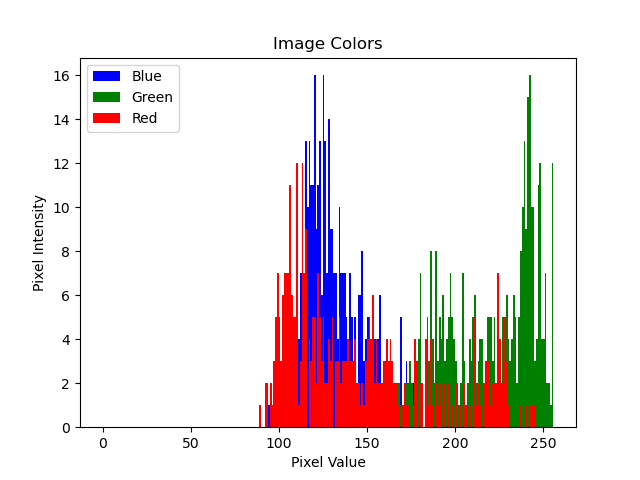
\includegraphics[width=.8\linewidth]{./Figures/green_hist.png}  
    	\caption{Histogram of green buoy.}
	\end{subfigure}
	\begin{subfigure}{.5\textwidth}
		\centering
		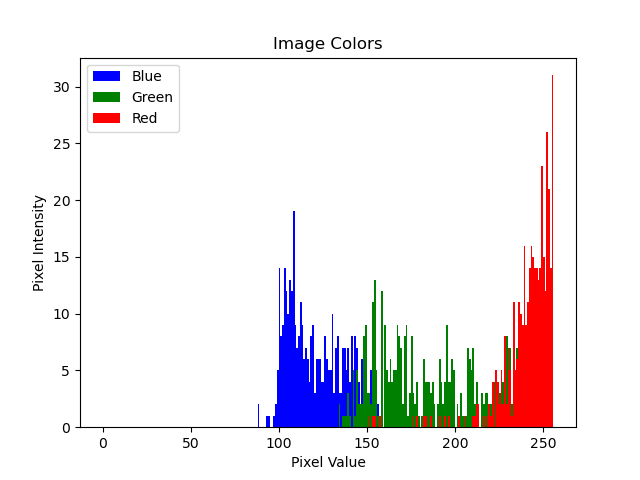
\includegraphics[width=.8\linewidth]{./Figures/red_hist.PNG}
		\caption{Histogram of orange buoy.}
	\end{subfigure}
	\begin{subfigure}{.5\textwidth}
		\centering
		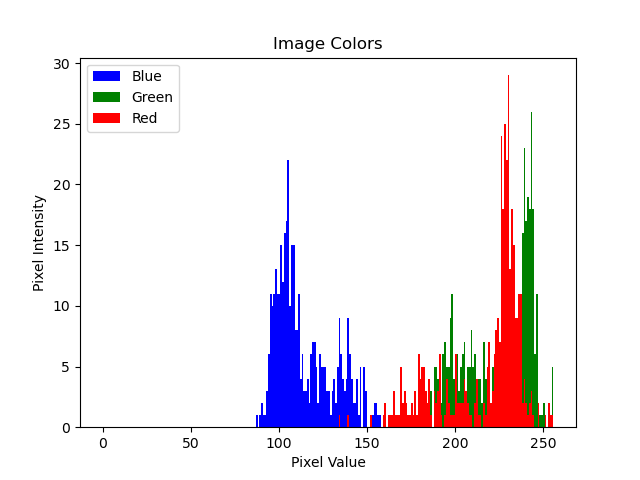
\includegraphics[width=.8\linewidth]{./Figures/yellow_hist.PNG}
		\caption{Histogram of yellow buoy.}
	\end{subfigure}
\end{figure}

Each buoy can be identified by the spike in the mid 200 range on the histograms. For the green buoy, the mean green color was just below 250. For the orange buoy, the mean red color was pretty much at 255. In order to threshold these two, we calculated the 1D Guassian of each histogram. This output gave us the mean and standard deviation of the color channel data. By using the mean and going half a standard deviation up and down, we were able to compute the upper and lower bounds of the threshold. Half a standard deviation was the decided value after multiple tests for thresholding the buoys. Figure (2a-b) shows the thresholded image of the green and orange buoys. For the yellow buoy, we had to use a combination of both the red and green channels. They were both between 230 and 240. We had to apply the 1D Guassian to both channels, threshold them separately using the mean and half of a standard deviation, and then use an AND statement for the two binary outputs. The final threshold can be seen in Figure (2c).

\begin{figure}[H]
	\begin{subfigure}{.5\textwidth}
		\centering		
		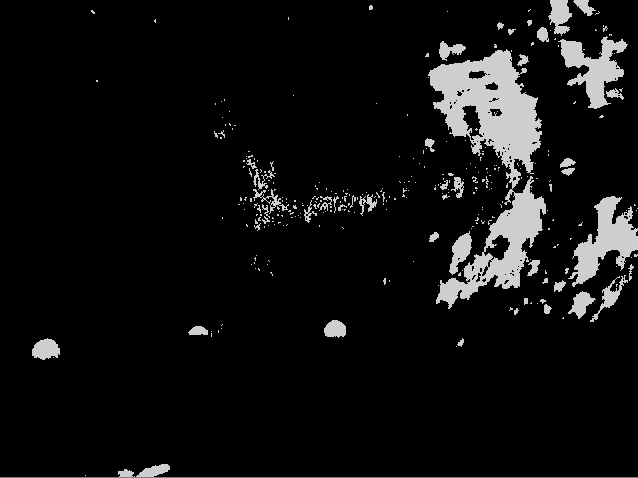
\includegraphics[width=.8\linewidth]{./Figures/green_thresh.PNG}  
    	\caption{Thresholded green buoy.}
	\end{subfigure}
	\begin{subfigure}{.5\textwidth}
		\centering
		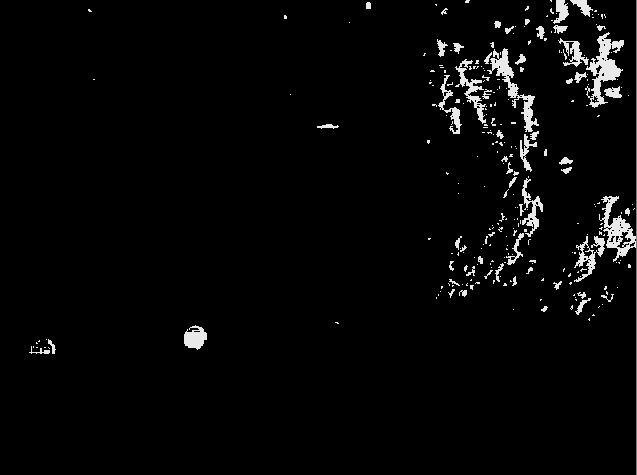
\includegraphics[width=.8\linewidth]{./Figures/red_thresh.PNG}
		\caption{Thresholded orange buoy.}
	\end{subfigure}
	\begin{subfigure}{.5\textwidth}
		\centering
		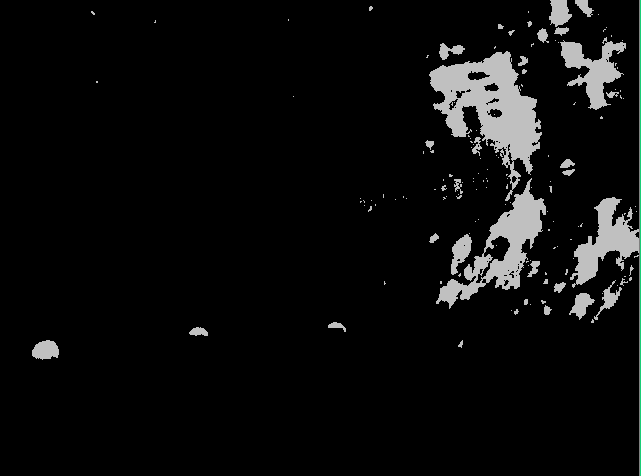
\includegraphics[width=.8\linewidth]{./Figures/yellow_thresh.PNG}
		\caption{Thresholded yellow buoy.}
	\end{subfigure}
\end{figure}


\part*{GMM and Maximum Likelhood Algorithm}

Using sample data, we used Expectation Maximization (EM) to find the Gaussian Mixture Model (GMM) for the probability densisty function. We used three 1-Dimensional Gaussians to put the separate the data into three different classes. This method of clustering the data into three separate local optimums is what allows us to determine what class it belongs to. Our GMM with three classes is shown below. Depending on the current value and where it lies in the data range, the algorithm determines what class it is in.

\begin{figure}[H]
	\centering		
	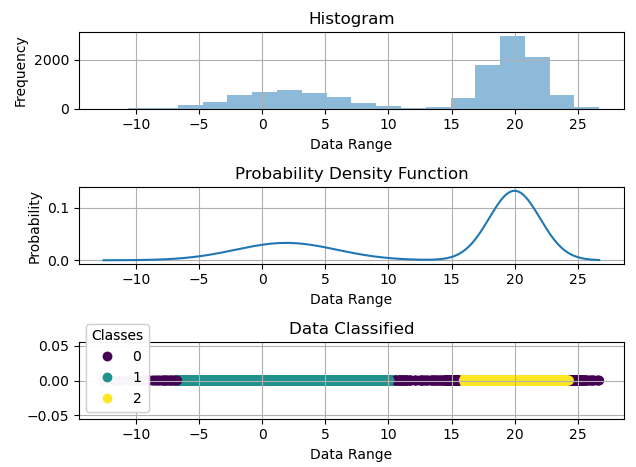
\includegraphics[width=.8\linewidth]{./Figures/GMM.PNG}  
    \caption{Plot of GMM wit 3 separate classes}
\end{figure}

For this specific chart, the mean and covariance of one of the clusters is provided below. 

\begin{equation}
	mean =  19.6\\
	covariance = 6.48
\end{equation}



\part*{Learning Color Models}
In order to figure out how many Gaussians [N] we needed, we looked at the histograms in Figure (3). Here we are showing green and yellow. Orange is the same as green because they are both close to a single color channel. Yellow is special because it is a combination of two color channels.

\begin{figure}[H]
	\begin{subfigure}{.5\textwidth}
		\centering		
		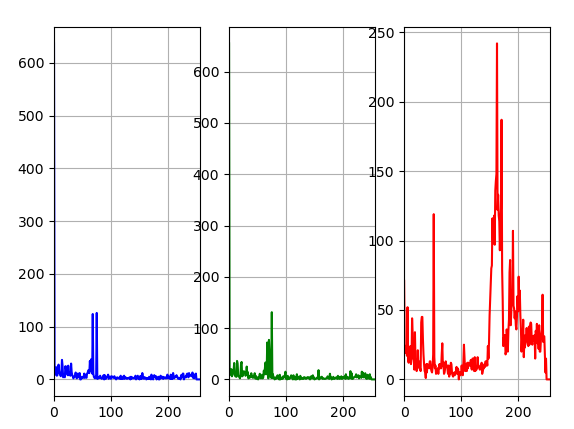
\includegraphics[width=.8\linewidth]{./Figures/yellow_hist2.PNG}  
    	\caption{Histogram of yellow buoy}
	\end{subfigure}
	\begin{subfigure}{.5\textwidth}
		\centering
		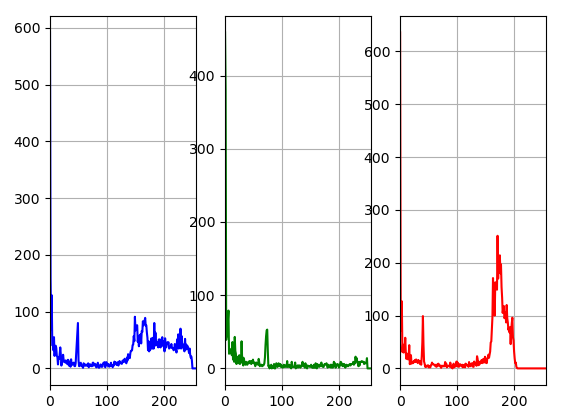
\includegraphics[width=.8\linewidth]{./Figures/green_hist2.PNG}
		\caption{Histogram of green buoy.}
	\end{subfigure}
\end{figure}

Based on this information and playing around with the data, we determined that the best number of Gaussians [N] is 3. This was the best fit for each buoy. The green and orange buoy both had dimensions of one while the yellow buoy had a dimension of two. This can be attritubted again to the fact that yellow is primarily two color channels. 

After implementing our EM algorithm, we found the mean and covariance of each cluster in our Gaussian distrubutions. In order to do this, we had to take the sample images we collected in section one and train our data on that. The twenty images we took for each buoy were then run through our EM algorithm we built. This code uses the training images and creates the Gaussian parameters that we later call upon to find the buoys. By training on the cropped buoy images, the [3]1-Dimensional Gaussian clusters move through every iteration of image until the three clusters find the local optimums. For an example, the final model parameters for the green buoy looked like as such.

\begin{equation}
	mean_{1} = 458 \\
	\begin{matrix}		
	covariance_{11} = 113459 cov_{12} = 82993 cov_{13}= 112323 \\
	covariance_{21} = 82993 cov_{22} = 60937 cov_{23}= 82319 \\
	covariance_{31} = 112323 cov_{32} = 82319 cov_{33}= 111338
	\end{matrix}
\end{equation}

This is one just one cluster out of three for the green buoy. After finding these parameters for every buoy color, we were able to create a visible model of the GMM. Depending on where the data falls on that chart, it is classified as that class.


\begin{figure}[H]
	\centering		
	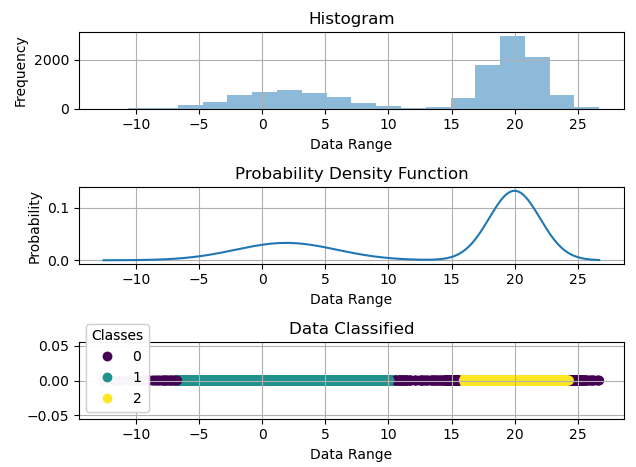
\includegraphics[width=.8\linewidth]{./Figures/GMM.PNG}  
    \caption{Plot of GMM wit 3 separate classes}
\end{figure}


\part*{Buoy Detection}

The final step is to string it all together by testing the models against each frame to detect the buoy and draw the contours around them.

This was done in a sequence of steps, leveraging the Gaussian Matrix Models that had been created earlier. First, a mask was created for each buoy to identify its location in the image frame. This was found by testing the model for each color buoy against the frame to determine which buoy in the frame best matched and then performing a series of erosions and dilations to remove noise and isolate the buoy. From this isolated image we were able to draw the bounding contours using OpenCV's built in findContours and drawContours functions. 

\begin{figure}[H]
	\begin{subfigure}{.5\textwidth}
		\centering		
		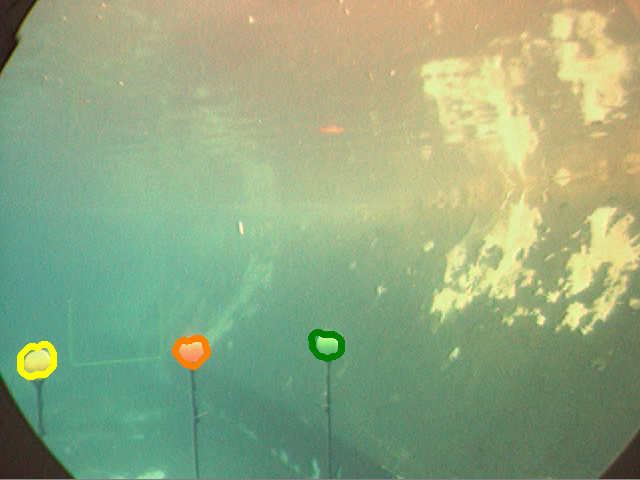
\includegraphics[width=.8\linewidth]{./Figures/Buoy1.PNG}  
    	\caption{A video frame with all three buoys}
	\end{subfigure}
	\begin{subfigure}{.5\textwidth}
		\centering
		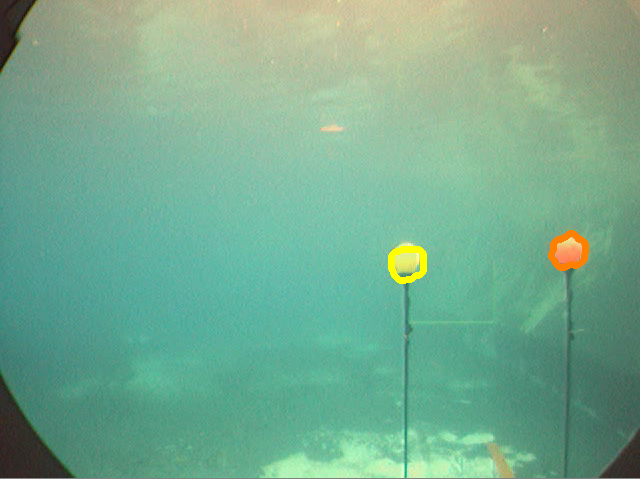
\includegraphics[width=.8\linewidth]{./Figures/Buoy2.PNG}
		\caption{A video frame with only the Yellow and Orange Buoys}
	\end{subfigure}
	\begin{subfigure}{.5\textwidth}
		\centering
		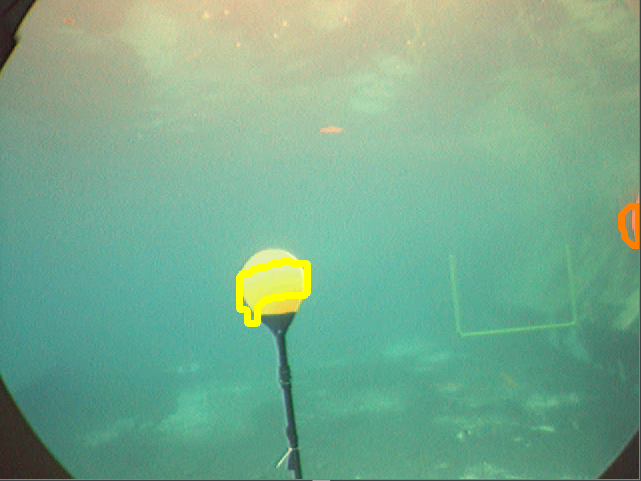
\includegraphics[width=.8\linewidth]{./Figures/Buoy3.PNG}
		\caption{A video frame with the Yellow Buoy and the Orange Buoy almost completely out of frame}
	\end{subfigure}
\end{figure}

We had some problems with the buoy detection at the end of the video. Becaus the camera is a lot closer to the buoys, the lighting changes the BGR values of the buoys. Becuase of this, the buoys don't fit into our Gaussian Mixture Model as well as they did in the previous frames. Only parts of the buoy show up in the binary image, so the contours are skewed and do not encompass the entire buoy. Perhaps better training data could have helped this problem. It was hard enough getting the current data we have and even harder getting it to localize at an optimum. Human error for data collection might be the cause of our algorithm's poor quality at the end.

The final output for our attempt at this project can be found online here: \url{https://youtu.be/WhunWTYdN7Q}

\end{document}
